\documentclass{article}

% my packages
\usepackage[utf8]{inputenc}
\usepackage[russian]{babel}
\usepackage{multicol}
\usepackage[14pt]{extsizes}
\usepackage[left=10mm, top=-1mm, right=5mm, bottom=10mm, nohead, nofoot]{geometry}
\usepackage{graphicx}
\graphicspath{{pictures/}}
\usepackage[usenames]{color}
\usepackage[most]{tcolorbox}
\usepackage{colortbl}
\usepackage{fancyhdr}
\pagestyle{fancy}
\fancyhf{}
\DeclareGraphicsExtensions{.png}
\usepackage{afterpage}
\fancyfoot[L]{40}
% document begins
\begin{document}
% make 2 columns
\begin{multicols}{2}

% insert picture with left-allignement
\begin{left}
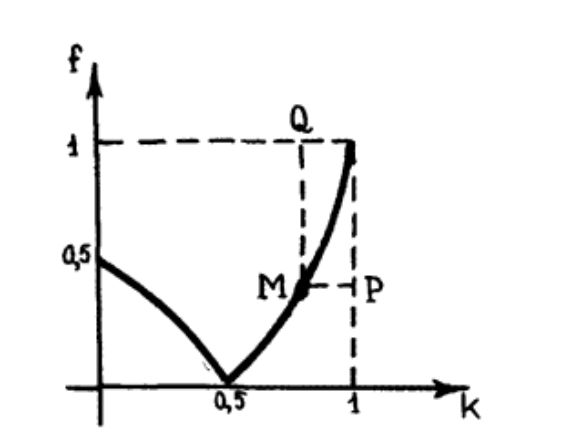
\includegraphics[scale=0.7]{pic.png}
\end{left}

% caption under the picture + text
\begin{small}
\parindent0pt Рис. 6. Пусть ${k_n=\frac{a_n}{b_n}}$. Тогда ${k_{n+1}=(k_n)}$, \\
где ${f(k)=\frac{|1-2k|}{2-k}}$. Здесь изображён график \\
этой функции на отрезке $0\leq k\leq1$. При реше- \\
нии задачи мы пользуемся тем, что для любой \\
точки $M$ правой половины графика \begin{scriptsize} $MQ/MP>2;$ \end{scriptsize} \\
если $0\leq k\leq\frac{1}{2}$, то $0\leq f(k)\leq \frac{1}{2}$, причём \\
$f(f(k))=k$, то есть функция $f$ на отрезке \\
$0\leq k\leq\frac{1}{2}$ совпадает с обратной к ней функци- \\
ей и график её симметричен относительно \\
биссектрисы угла между осями координат. \\
\hfill 
\end{small}
% caption end

% table start
\renewcommand{\arraystretch}{1.5}
\parindent0pt\begin{tabular}[b]{ | m{0.4cm} | m{0.4cm} | m{0.4cm} | m{0.4cm} | m{0.4cm} | m{0.4cm} | m{0.4cm} | m{0.4cm} | m{0.4cm} | }
\hline
$ $ & $ $ & $ $ & $ $ & $ $ & $ $ & $ $ & $ $ & $ $ \\ \hline
$ $ & $ $ & $ $ & $ $ & $ $ & $ $ & $ $ & $ $ & $ $\\ \hline
$ $ & $ $ & $\text{-}\frac{1}{2}$ & $\frac{1}{2}$ & $ $ & $\frac{1}{2}$ & $\text{-}\frac{1}{2}$ & $ $ & $ $ \\ \hline
$ $ & $ $ & $ $ & $ $ & $ $ & $ $ & $ $ & $ $ & $ $\\ \hline
$ $ & $ $ & $\frac{1}{2}$ & $\text{-}1$ & $ $ & $\text{-}1$ & $\frac{1}{2}$ & $ $ & $ $\\ \hline
$ $ & $ $ & $\text{-}1$ & $1$ & $1$ & $1$ & $\text{-}1$ & $ $ & $ $\\ \hline
$ $ & $ $ & $\frac{1}{2}$ & $\text{-}1$ & $ $ & $\text{-}1$ & $\frac{1}{2}$ & $ $ & $ $\\ \hline
$ $ & $ $ & $ $ & $ $ & $ $ & $ $ & $ $ & $ $ & $ $\\ \hline
$ $ & $ $ & $\text{-}\frac{1}{2}$ & $\frac{1}{2}$ & $ $ & $\frac{1}{2}$ & $\text{-}\frac{1}{2}$ & $ $ & $ $ \\ \hline
$ $ & $ $ & $ $ & $ $ & $ $ & $ $ & $ $ & $ $ & $ $\\ \hline
$ $ & $ $ & $ $ & $ $ & $ $ & $ $ & $ $ & $ $ & $ $\\ 
\hline
\end{tabular}
\renewcommand{\arraystretch}{1}
% table end

% caption under the table
Рис. 7. Во всех незаполненных клетках \\
стоят нули.
\par

% text
\setlength{\parindent}{15pt} Во-вторых, если $\frac{a_n}{b_n}>\frac{1}{2}$, то \\
\begin{large}
\setlength{\parindent}{10pt}
\indent $\frac{1-\frac{a_{n+1}}{b_{n+1}}}{1-\frac{a_n}{b_n}}=\frac{1-\frac{2a_n-b_n}{2b_n-a_n}}{1-\frac{a_n}{b_n}}=$\\
\\
\setlength{\parindent}{90pt} 
\indent $=\frac{3b_n}{2b_n-a_n}>\frac{3b_n}{2b_n-\frac{b_n}{2}}=2;$
\end{large}


%text on next column
\setlength{\parindent}{0pt} 
\indent 
\\
\\
таким образом, величина $1-\frac{a_n}{b_n}$ при\\
переходе от $n$ к $n+1$ увеличивается\\
не менее чем в два раза до тех пор,\\
пока мы не придём к прямоугольнику\\
с $\frac{a_n}{b_n}\leq\frac{1}{2}$. Поэтому, каким бы ма-\\
лым ни было $1-\frac{a_1}{b_1}$, всегда после\\
нескольких - не более чем $-1-$\\
$-log_2 (1-\frac{a_1}{b_1})-$ операций мы придём\\
к прямоугольнику второго типа, и\\
дальше в нашей последовательности\\
будут встречаться только такие пря-\\
моугольники.

\setlength{\parindent}{22pt} 
\indent Поэтому мы можем считать, что\\
уже $\frac{a_1}{b_1}<\frac{1}{2}$.\\
\indent При этом\\
$a_3=b_2-2a_2=$\\
\setlength{\parindent}{45pt}
\indent $=(2b_1-a_1)-2(b_1-2a_1)-3a_1$,\\
\setlength{\parindent}{0pt}
\indent $b_3=2b_2-a_2$\\
\setlength{\parindent}{40pt}
\indent $=2(2b_1-a_1)-(b_1-2a_1)=3b_1$.\\

\setlength{\parindent}{0pt} 
\indent Следовательно, вообще $a_{2k+1}=3^ka_1$\\
И $b_{2k+1}=3^kb_1$, причём сумма чисел\\
в этом прямоугольнике $3^ka_1\times3^kb_1$\\
больше $4+9^k\epsilon$, то есть, выбрав k\\
достаточно большим, мы можем сде-\\
лать ее сколько угодно большой. Те-\\
перь уже нетрудно получить проти-\\
воречие: ясно, что любой прямоуголь-\\
ник $Na_1\times Nb_1$, где $a_1$, $b_1$ и N - \\
целые числа, можно разбить на $a_1b_1$\\
квадратов (со стороной N), и поэтому\\
сумма чисел в нем не может превос-\\
ходить по модулю числа $a_1b_1$.\\
\setlength{\parindent}{20pt} 
\indent Рисунок 6 поясняет вторую поло-\\
вину доказательства. На рисунке 7\\
изображён пример, для которого сум-\\
ма чисел в некотором прямоуголь-\\
нике равна трём. Таким образом, для\\
$c=2$ утверждение задачи неверно. \\
Весьма правдоподобно, что точная\\
оценка $c=4$, но примеров, показы-\\
вающих, что $c>3$, мы не знаем.\\
\\
\setlength{\parindent}{130pt} 
\indent \emph{Н. Б. Васильев}
\end{multicols}
\end{document}